\appendix

\section{Additional Details}
\subsection{Correction Factor}
\label{correction_factor}
$\hat{P}_{noise}$ is the probability that a sample $x \in X$ can have noise in its label and $\eta$ is the noise or probability that a label is flipped. Also, let P be the true probability that a label is 1, then we can consider two scenarios
\begin{itemize}
    \item The true label is 1 and is not flipped $\left(P(1-\eta)\right)$
    \item The true label is 0 and is flipped $\left((1-P)\eta\right)$
\end{itemize}
\begin{align*}
    \hat{P}_{noise} &= P(1-\eta) + (1-P)\eta \\
    \hat{P}_{noise} &= P - P\eta + \eta - P\eta \\
    \hat{P}_{noise} - \eta &= P(1 - 2\eta) \\
    P &= \frac{\hat{P}_{noise} - \eta}{1 - 2\eta} \\
\end{align*}

This value is the correction factor and represents the proportion of labels that are not affected by the label noise.

\subsection{Algorithm Results}
\label{app:algo_analysis}
In this section, we give the results of the experiments conducted using the algorithm proposed in Section \ref{sec:implementation}. We conducted three types of experiments by varying $\epsilon, \tau \text{ and } \eta$. For each of the experiments, we fixed $min=-100 \text{ and } max=100$. We run each algorithm $150$ times to reduce the effect of stochasticity. Figure \ref{fig:results} shows the average number of statistical queries used by the algorithm for each of the different values of $\delta^{-1}$ along with $95\%$ confidence interval. For the first experiment, we varied the value of $\epsilon$, and kept $\tau$ and $\eta$ fixed at $0.1$ and $0.05$, respectively. Figure \ref{fig:epsilon} shows that for bigger values of $\epsilon$ it takes fewer queries to converge which was expected as convergence is faster for more error. For the second experiment, we varied $\tau$ and fixed $\epsilon=0.05$ and $\eta=0.05$. As shown in Figure \ref{fig:tau}, for $\tau=0$ it took comparatively too many queries for the algorithm to converge. This might be because for $\tau=0$ the algorithm became very prone to the noise in the data. For the last experiment, we varied $\eta$, and kept $\epsilon=0.05$ and $\tau=0.1$. In this case, as noise increased more queries were needed by the algorithm to find the hypothesis function. The algorithm also took very few queries in the noise-free situation (Figure \ref{fig:eta}). The analysis given in Section \ref{algo_analysis} gave the theoretical upper bound for the random search algorithm but it is worth noting that the experimental results show that the resultant algorithm is comparatively very optimal. This is because the proposed algorithm even though it initializes the initial hypothesis function randomly and searches through the concept class randomly but the search is guided by the output of the statistical query oracle ($\nu$). Based on $\nu$, the hypothesis function is only updated when the resultant change will make it closer to the resultant rectangle, in turn, making the algorithm efficient. The experiment code is available at \url{https://github.com/aniketsharma00411/statistical_query_learning}.

\begin{figure*}
    \centering
    \subfigure[]{
        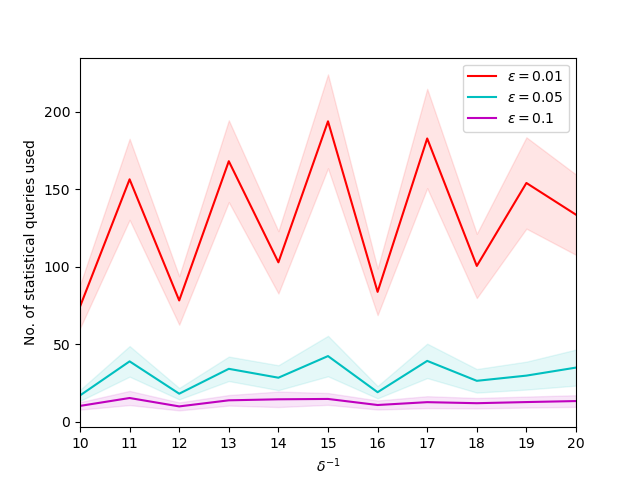
\includegraphics[width=0.48\textwidth]{report/figs/epsilon.png}
        \label{fig:epsilon}
    }
    \subfigure[]{
        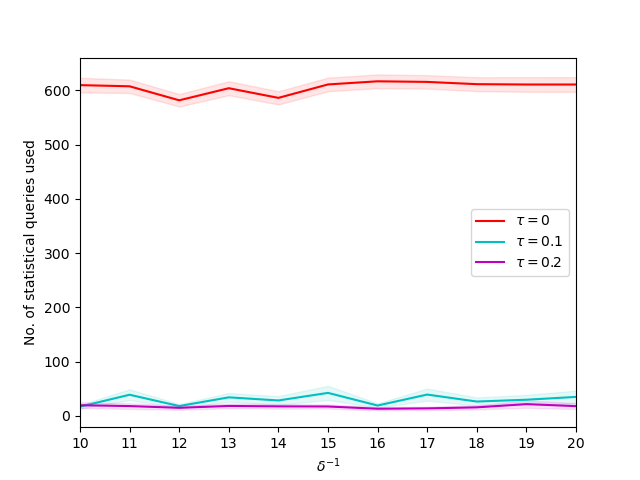
\includegraphics[width=0.48\textwidth]{report/figs/tau.png}
        \label{fig:tau}
    }
    \subfigure[]{
        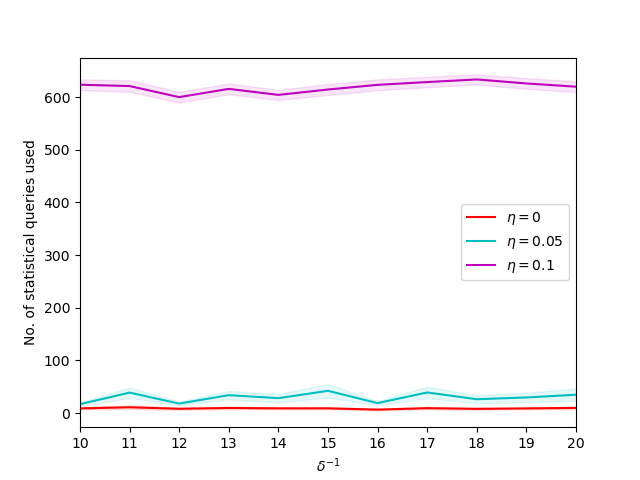
\includegraphics[width=0.48\textwidth]{report/figs/eta.png}
        \label{fig:eta}
    }
    \caption{Number of queries needed by the algorithm for (a) $\epsilon \in \{0.01, 0.05, 0.1\}, \tau=0.1, \eta=0.05$ (b) $\tau \in \{0, 0.1, 0.2\}, \epsilon=0.05, \eta=0.05$ (c) $\eta \in \{0, 0.05, 0.1\}, \epsilon=0.05, \tau=0.1$}
    \label{fig:results}
\end{figure*}